\section{Introduction}
Acquisition of DWB datasets in Step and Shoot mode, using overlapping beds, results in a complex dataset of pet RAW data in relation to timing and positional information. Moreover, the addition of an initial dynamic single bed acquisition, commonly conducted for IDIF derivation purposes, can enrich the dataset and allow for more complex kinetic modeling of the sampled region~\cite{Zaker2020} but increases the complexity of the whole examination pet RAW dataset. 

Suggested practices~\cite{Karakatsanis2013} and state of the art implementations~\cite{Hu2020} of DWB protocols regard the two datasets (DSB and DWB) as independent and suggest to perform independent reconstructions on each dataset. Post reconstruction kinetic model fitting can then combine the reconstructions result TAC information over the two datasets and make use of the complete acquisition information. 
Furthermore, the DWB dataset will contains information over the overlapping bed regions that will be sampled for longer compared to central regions if the bed positions in order to increase sensitivity at the bed edges. But the result is different timing information for locations that fall at the overlapping regions, compared to other body locations. In post-reconstruction kinetic modeling, which is applied independently on each voxel TAC, suggested practices make use of modified timing information (average of two bed position timings) for voxels that fall in overlapping regions~\cite{Karakatsanis2013}. 
For use of the DWB data with dynamic reconstruction the independent reconstruction of bed positions and post-reconstruction overlapping of result parametric images has been suggested~\cite{Karakatsanis2016a}, similar to that conducted in static WB imaging~\cite{Schubert1996}.
It is important to note that DWB acquired in CBM mode, although free of the need of overlapping bed acquisitions requires similar timming considerations to be taken into account for each axial location of the DWB acquisition~\cite{Karakatsanis2016b,Hu2020}.

The flexibility offered by the CASToR reconstruction platform allows for the concept of direct reconstruction of multi-bed data~\cite{Ross2004} to be expanded to DWB data, where the exact timing information of the dataset and all bed positions can be used within the iterative reconstruction loop of dynamic reconstruction. Furthermore the offered flexibility can allow for combination of the DSB and DWB datasets to be used within the same reconstruction loop. 
In this chapter we describe how this novel DWB protocol reconstruction concept was implemented in CASToR and present results from dynamic reconstruction of DWB data of the IsotoPK study, as presented in the EANM2020 conference~\cite{chalampalakis2020EANM}.
Finally we discuss the complications arising from kinetic model fitting errors in dynamic reconstruction and their importance for DWB reconstruction. We present our work towards reduction of these errors using adaptive residual modelling for dynamic reconstruction, as presented in the IEEE-MIC2020 conference~\cite{}.

\section{Methods}

An example of a three bed positions DWB protocol is given in figure~\ref{fig_3_3:OverlapFraming} to describe the nature of the timing information of the overlapping regions of such data. The bed locations and amount of overlapping region in this example are identical to the setup used for the NHP acquisition on the Signa PET/MR, described in chapter ~\ref{Chap3_1:AcquisitionOptimization}.
As it can be seen at the left diagram of figure~\ref{fig_3_3:OverlapFraming} axial positions that fall outside of the overlap region result in framing that is equal to the framing of their respective bed positions. Positions over the overlap regions, seen at the right diagram of figure~\ref{fig_3_3:OverlapFraming}, result in framing equal to that of both used bed positions, which is twice the number of frames compared to locations outside the overlap. Moreover, locations at the overlap are not sampled continuously from both contributing bed positions due to the interruption by the movement of the bed and system delays.  
Finally the complexity is increased when a dynamic single bed phase is included, as shown in  figure~\ref{fig_3_3:CompleteProtocolFraming}, with initial frames from DSB contributing to different locations of the DWB acquisition that might fall in overlap regions or not depending on the protocol setup. 

\begin{figure} [h!]
\centering
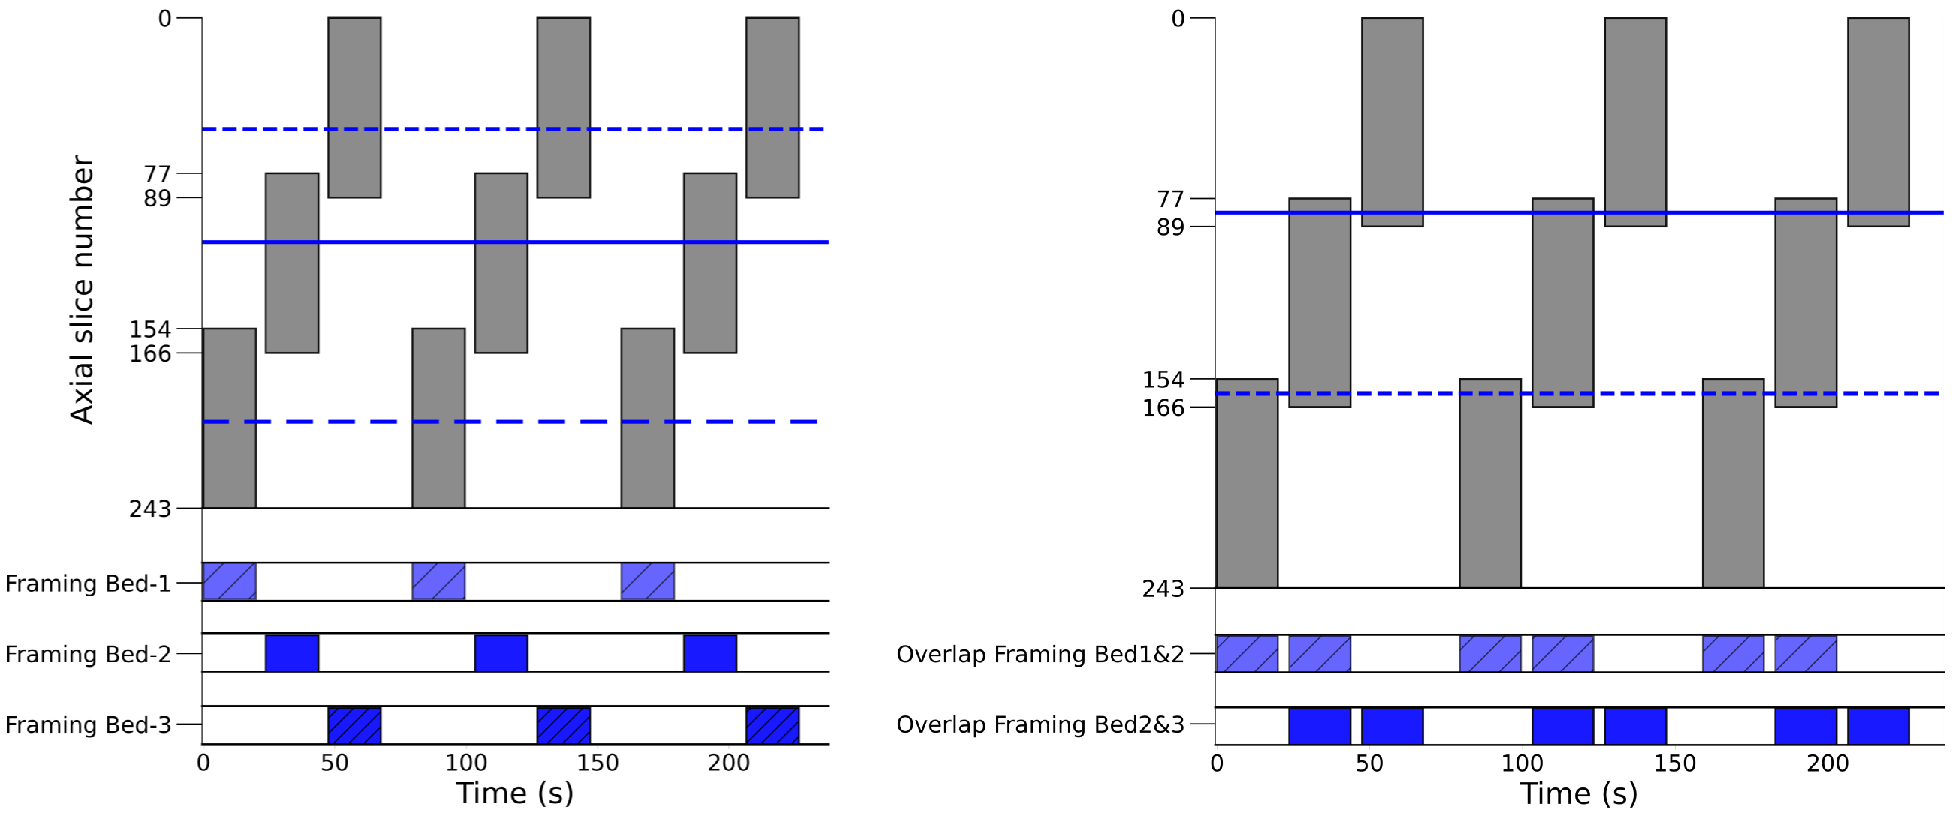
\includegraphics[scale=0.50,angle=0]{3_Results/3_3_DWB_Reconstruction/figures/OverlapTiming.pdf}
\caption{} 
\label{fig_3_3:OverlapFraming}
\end{figure} 

\begin{figure} [h!]
\centering
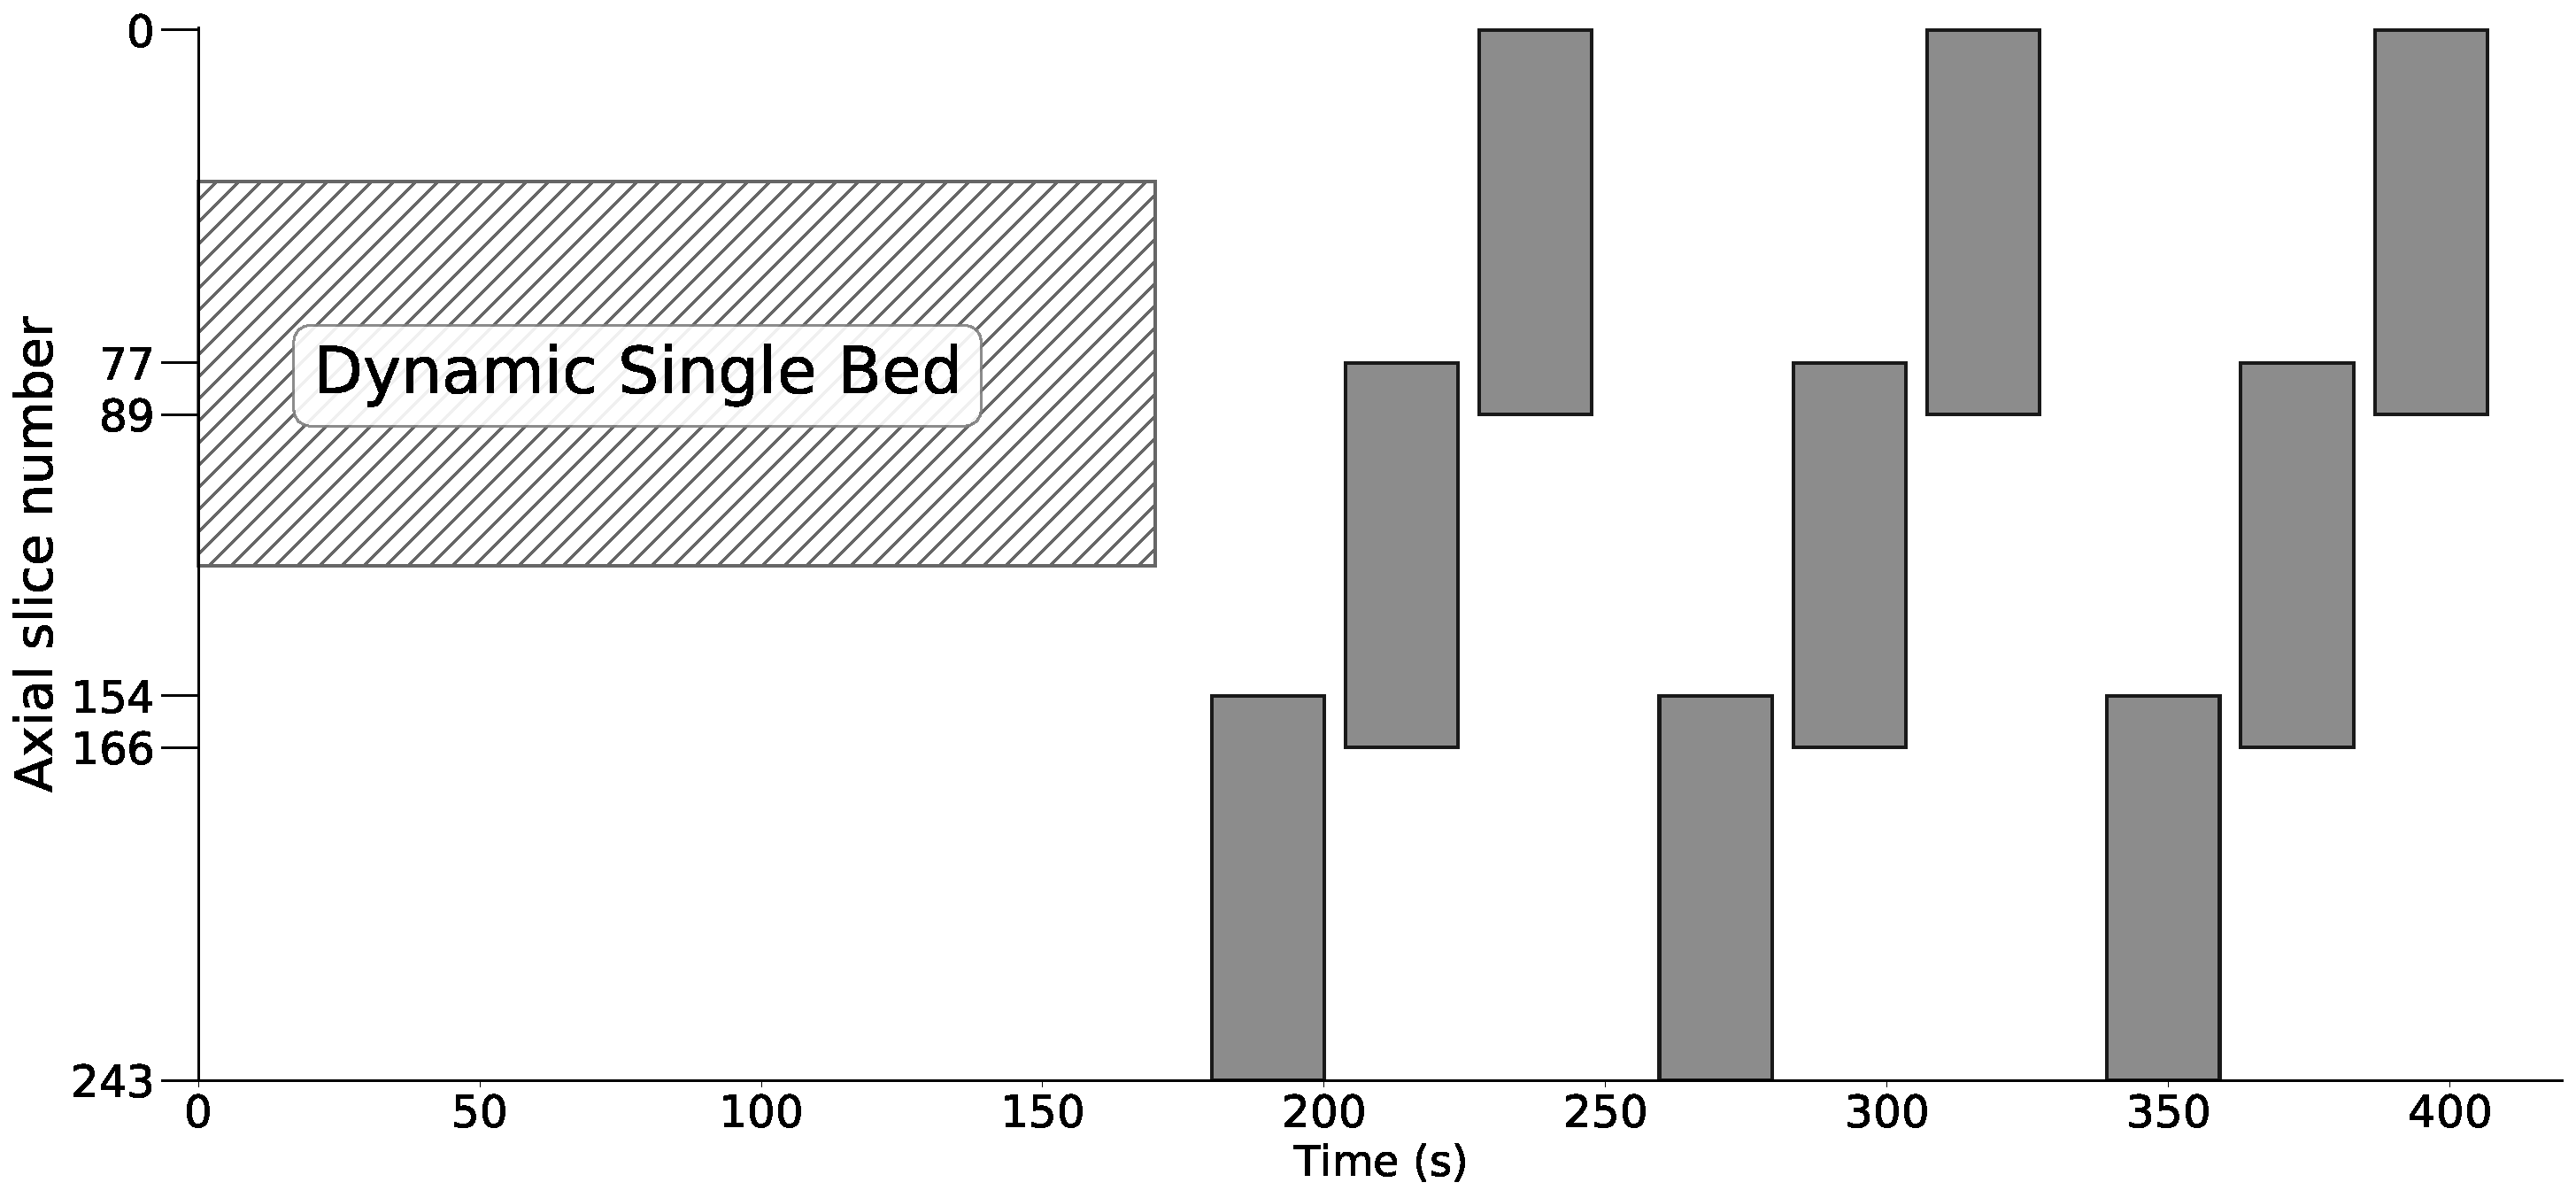
\includegraphics[scale=0.28,angle=0]{3_Results/3_3_DWB_Reconstruction/figures/CompleteProtocolTiming.pdf}
\caption{} 
\label{fig_3_3:CompleteProtocolFraming}
\end{figure} 

If we consider only the DWB dataset and do not split each individual Step and Shoot acquisitions into multiple frames, then the total number of frames in the DWB dataset will be defined by all the individual Step and Shoot acquisitions. In the example presented in figure~\ref{fig_3_3:OverlapFraming} the DWB data provide nine frames. 
But not all frames need to be considered for each of the three bed positions or for locations at the overlapping regions. 
The choice of the appropriate frames for each location in image space, whether within or outside the overlap, can be made using an mask that indicates which locations are sampled on each frame. 
This type of mask could be used for post-reconstruction parametric imaging that relies on estimation of kinetic models on each voxel's TAC. 

With CASToR the use of multi-bed data can be made directly within its unique iterative loop, using the methodology described in section~\ref{chap2_4:MultiBedRecon}. The same framework can be extended to dynamic reconstruction of DWB datasets within the same iterative loop. Specifically in dynamic reconstruction where a dynamic model is applied over the frames of the acquisition, the model will consider all frames of the DWB acquisition. But incorporation of the bed offset information in the projection operation for each voxel $j$ will naturally lead to the selection of frames that correspond to the sampled time points for the location of voxel $j$ in the DWB dataset.
In the case of dynamic reconstruction using linear models, we description provided above can be shown by combining equations~\ref{eqn:4DMLEM} and ~\ref{eqn2_4:MLEM_multibed}. \textbf{We can incorporate the positional information of each bed offset into the frame depedent information of the projection $P$}

This provides

\begin{equation}
\theta_{pj}^{(k+1)} = \frac{\theta_{pj}^{(k)}}
{\sum_{t=1}^{n_t} B_{tp} \sum_{i=1}^{n_i} P_{tij}} 
\sum_{t=1}^{n_t} B_{tp}  \sum_{i=1}^{n_i} P_{tij} 
\frac{y_{ti}}
{\sum_{d=1}^{n_j} P_{tid} \sum_{p=1}^{n_p} B_{tp}\theta_{pj}^{(k)} + B_{ti} } \\, \\
\label{eqn:4DMLEM_Multibed}
\end{equation} 
\textbf{Not sure this is correct with the separation of time and beds}!

where the set of basis functions $B$ is precomputed for all time frames $t$ of the DWB acquisition, but is effectively applied in each voxel $j$ for the time frames that are not masked by the back-projection operation $\sum_{t=1}^{n_t} \sum_{i=1}^{n_i} P_{tij}$. It is important to note that with this operation there is no additional need for consideration of overlapping after reconstruction and parametric images $\boldsymbol\theta$ have dimensions of the effective FOV. 

Use of this framework to perform individual frame reconstructions is also permitted, where matrix $\boldsymbol{B}$ will be the identity matrix meaning that frame reconstructions will be independent of each other. This will be equivalent to performing the following reconstruction for each frame $t$. 
An example from the use of this framework for frame reconstructions is shown in figure~\ref{fig_3_3:Macaque} for a group of three consecutive frames. The sensitivity images for the same frames, as estimated by the back-projection operation $\sum_{t=1}^{n_t} \sum_{i=1}^{n_i} P_{tij}$, are shown in figure~\ref{fig_3_3:Macaque_Sensitivity}.
The sensitivity images clearly show the sampled locations per frame and the overlapping locations for adjacent frames. 
%In this three bed acquisition a total of 243 axial slices are allocated in image space per frame, from which 89 will be sampled at each frame and bed. The overlap locations, in this case for 12 axial slices, which are sampled over consecutive frames can be identified from the frames sensitivity image. 
Individual frame reconstruction of DWB data, using the effective FOV and by accounting for the bed offset in image space, can easily be used for post-reconstruction kinetic model fitting without the need for considerations on bed positions after reconstruction. In addition for post-reconstruction kinetic model fitting, the result sensitivity frame images can be used as a mask for the dynamic model as described above. 

%
\begin{figure} [h!]
%\centering
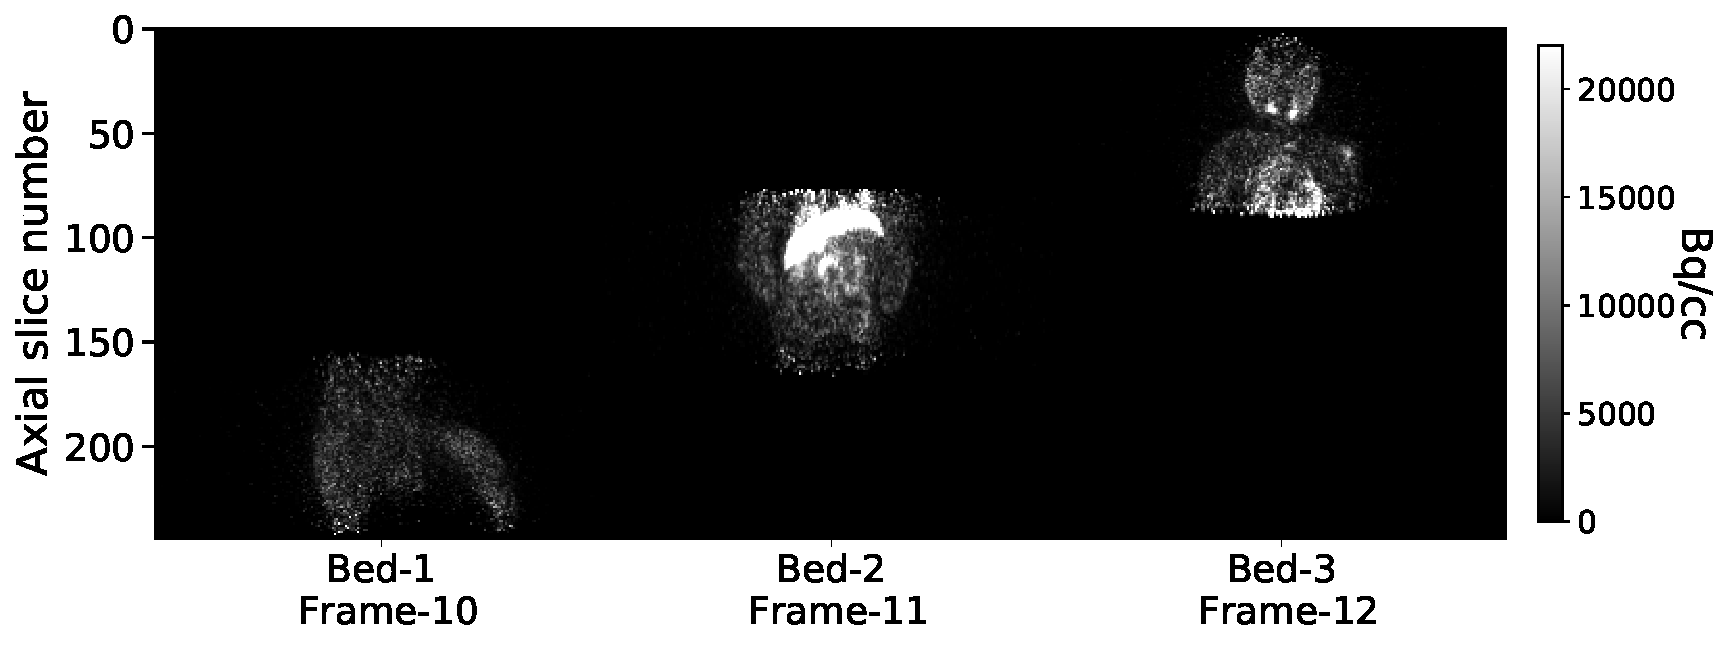
\includegraphics[scale=0.5,angle=0]{3_Results/3_3_DWB_Reconstruction/figures/Macaque_3D.pdf}
\caption{Example three frame image from a three bed positions DWB acquisition.} 
\label{fig_3_3:Macaque}
\end{figure} 
%
\begin{figure} [h!]
%\centering
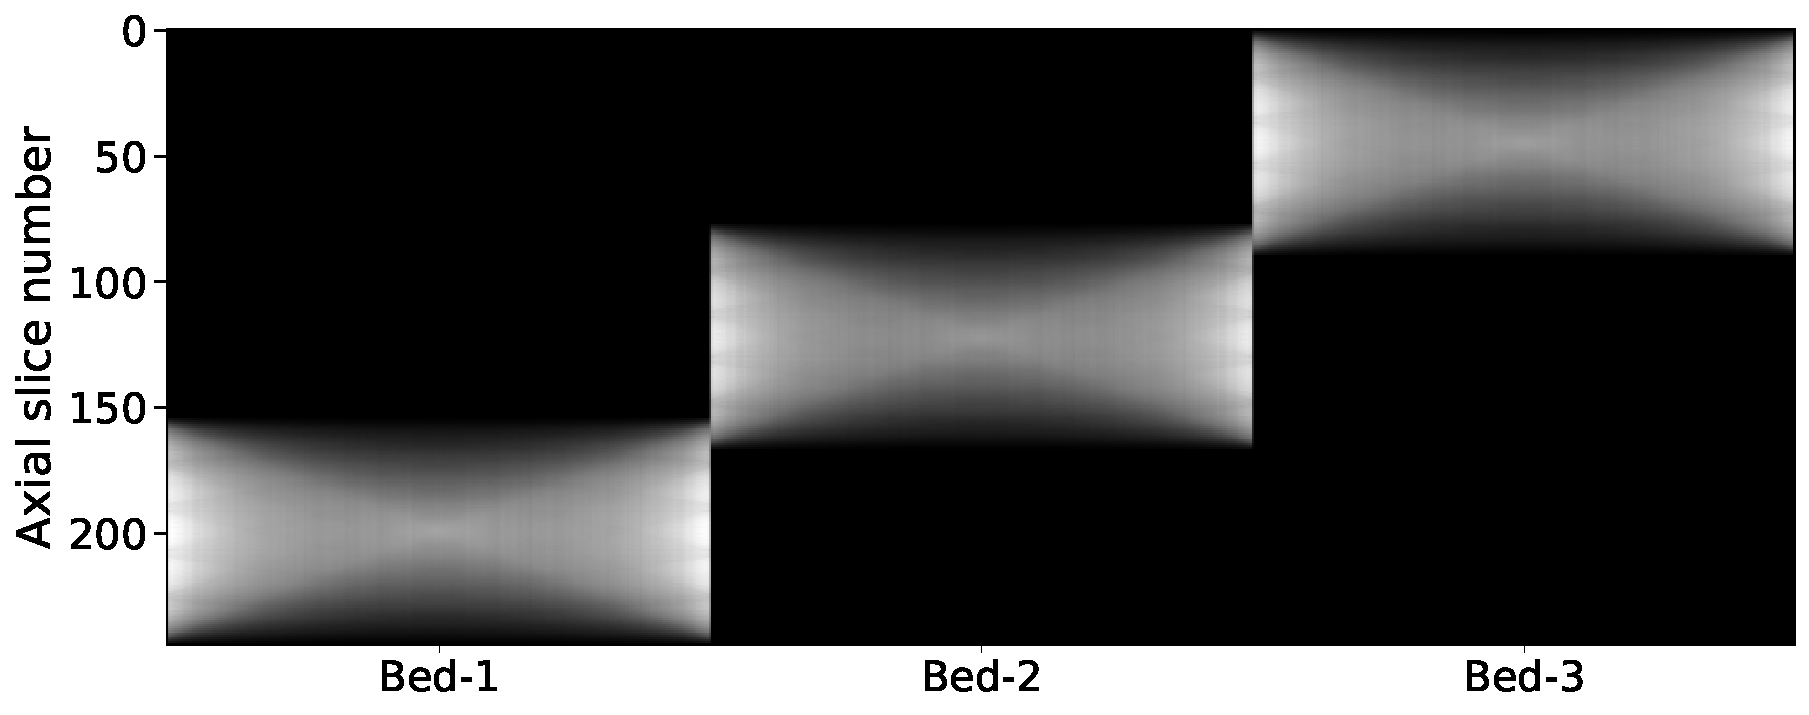
\includegraphics[scale=0.42,angle=0]{3_Results/3_3_DWB_Reconstruction/figures/Macaque_Sensitivity.pdf}
\caption{Example three frame sensitivity image from a three bed positions DWB acquisition.} 
\label{fig_3_3:Macaque_Sensitivity}
\end{figure} 
%

The described methodology for direct multi-bed dynamic reconstruction and its offered flexibility allows for any sequence of the acquired bed/frames to be used within the iterative reconstruction loop. Furthermore, the use of the DSB dataset can also be included in the iterative loop while also bee divided into multiple shorter frames.

\subsection{Considerations for Nested Optimization}
For use of multi-bed dynamic reconstruction under the nested optimization framework, additional considerations need to be made.
The nested optimization framework decouples the dynamic model fitting process on image space data from the tomographic update process over the raw PET data. The two steps are conducted with an MLEM update over the PET raw data using equation~\ref{eqn:EM_Update_image} to get the EM update image for all frame data, followed by kinetic model fitting by optimisation of the likelihood function of equation~\ref{eqn:NestedOptimization}. 
For linear models the likelihood function over image TAC data can be written as equation~\ref{eqn:NestedOptimization}, which for single bed dynamic studies can be optimised using the image based MLEM update of equation~\ref{eqn:NestedEM}.
This derivation ignores the sensitivity factor of the original likelihood function, as it assumes that the sensitivity of a voxel over the TAC is the same and thus can be ignored in the optimisation process. 
But this is not necessarily the case at the overlap locations of DWB datasets. 
For direct multi-bed reconstruction of DWB data the two step process needs to be modified to

\begin{equation}
\label{eq3_3:NestedMultibed}
\text{}
\begin{cases}  
f_{tj}^{(EM)} = \frac{f_j(\bm\theta^{(k)})}{\sum_{i=1}^{n_i} P_{tij}} 
\sum_{i=1}^{n_i} P_{tij} 
\frac{y_{ti}}{\sum_{d=1}^{n_j} P_{tid} f_d(\bm\theta^{(k)}) + B_{ti} } \\ \\
\argmax{\bm{\theta}} 
\sum_{t=1}^{n_t} \sum_{b=1}^{n_j} \left[ \sum_{i=1}^{n_i}  P_{tib} \right]
\left[ -f_b(\bm\theta^{(k)}) + 
ln( f_b(\bm\theta^{(k)})) 
f_{tb}^{(EM)}(\bm{\theta}^{(k)})
\right] .\\
\end{cases}
\end{equation}

The tomographic update of this two-step optimization process is effectively an update over the DWB data for independent frame reconstruction, similar to the process described for the NHP example above. The second step is an image space optimization process that now needs to consider the sensitivity $\sum_{s=1}^{n_s} \sum_{i=1}^{n_i}  P_{sib}$ of each time point $t$ in the TAC of each voxel. For linear models, where before an image based MLEM algorithm was used for this image space optimization process, an weighted MLEM update can be used with the sensitivity of each time point $t$ as the weight. Or alternatively non-linear optimization algorithms can be used for non-linear dynamic models estimation, by making use of weighted optimization with the same sensitivity values.

\iffalse 
\begin{equation}
\theta_j^{(k+1)} = \frac{\theta_j^{(k)}}
{\sum_{p=1}^{n_p} w B_{pj}} 
\sum_{p=1}^{n_p} w B_{pj} 
\frac{f_{j}^{(EM)}(\bm{\theta}^{(k)})}{\sum_{d=1}^{n_j} B_{pd}\theta_d^{(k)} } \\.
\label{eqn3_3:WeightedNestedEM}
\end{equation}
\fi

\section{Results}

\subsection{IsotoPK-Study}



\section{Discussion}
We have presented a framework for direct multi-bed reconstruction of DWB datasets, for individual frame reconstruction as well as dynamic reconstructions. The flexibility offered by this framework and by the CASToR reconstruction platform allows for the use of the DSB data that are commonly acquired prior to DWB acquisition, in the same reconstruction loop. We have shown how the framework can be extended for use with nested optimization for dynamic reconstruction.

We performed an inconclusive evaluation study with the NHP dataset by splitting the acquired data into 10 replicates, to evaluate differences between the post-reconstruction overlapping of parametric image and direct multi-bed DWB reconstruction of parametric images. But results were inconclusive and showed the need for a detailed simulation study to assess differences in terms of bias and noise properties of the overlapping regions. 
